\documentclass[a4paper]{report}
\usepackage[T1]{fontenc}
\usepackage[utf8]{inputenc}
\usepackage[english]{babel}
\usepackage{geometry}
\usepackage{graphicx}
\usepackage{subfig}
\geometry{a4paper,top=2.5cm,bottom=2.5cm,left=3cm,right=3cm,%
	heightrounded,bindingoffset=5mm}
\begin{document}

\title{\Huge{JustRecipe}}
\author{\Large{Francesco Campilongo - Daniele Cioffo - Francesco Iemma}}
\date{Academic Year 2020/21}
\maketitle
\tableofcontents

\chapter*{Introduction}

\chapter{Dataset}


\chapter{Design}
\section{Introduction To The Application}
\section{Requirements}
\subsection{Main Actors}
\subsection{Functional Requirements}
Unregistered User
\begin{itemize}
	\item Sign-up
\end{itemize}
User
\begin{itemize}
	\item Login/Logout
	\item Search a recipe
	\item Browse suggested recipes
	\item Browse recipes of following users
	\item Add a recipe
	\item Edit own recipes
	\item Comment recipes
	\item Follow another user
	\item Like a recipe
\end{itemize}
Moderator
\begin{itemize}
	\item Delete comments
\end{itemize}
Administrator
\begin{itemize}
	\item Delete users
	\item Delete recipes
	\item Elect moderators
\end{itemize}
\subsection{Non-Functional Requirements}

\subsection{Actors and Use Cases}
The use case diagram of the application is described in the figure 2.1 
\begin{figure}[htpb]
	\centering
	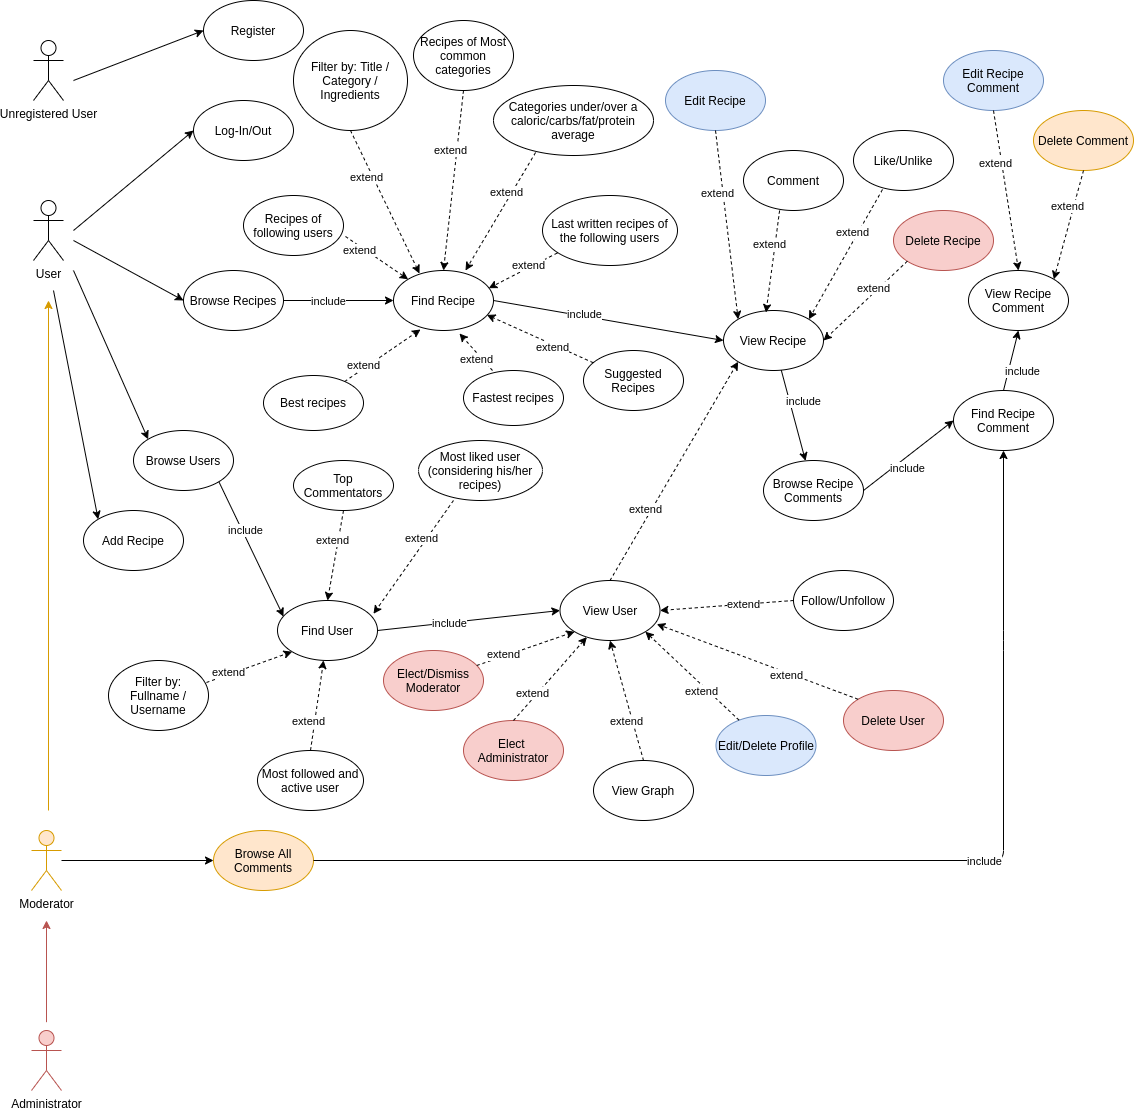
\includegraphics[scale=0.5]{img/UseCaseDiagram.png}
	\caption{Use Case Diagram}
\end{figure}
\section{UML Class Diagram}
\section{Data Model}
\subsection{DocumentDB}
\subsection{GraphDB}
\section{Distributed Database Design}
\subsection{Replicas}
\subsection{Sharding}
\section{Software Architecture}


\chapter{Implementation and Test}
\section{Main Modules}
\section{Main Packages and Classes}
\section{Most Relevant Queries}
\subsection{MongoDB}
\subsection{Neo4J}
\section{Unit Test}
\section{Tests and Statistical Analysis}

\chapter{User Manual}
\end{document}